%!TEX root = Algebraische_Zahlentheorie.tex

\renewcommand{\lecdate}{22.10.14}

\begin{Folgerung}
 $\IZ[i]$ ist ein HIR, also faktoriell.
\end{Folgerung}

\begin{Beweis}
 Sei $\Fa\subset \IZ[i]$ ein Ideal $\neq(0)$. $0\neq q\in \Fa$ von minimaler Norm. Dann gilt: $(q)\subset\Fa$. Sei $m\in \Fa$, $m=xq+r$ mit $r\in\Fa$ und $0\leq N(r)<N(q)$. 
 Es folgt $r=0$, also $m\in(q)$.
\end{Beweis}

\begin{Bemerkung}
 \begin{itemize}
  \item $\IZ[i]$ hat die gleiche Arithmetik wie $\IZ$: $\ggT$ (Eindeutig bis auf Einheiten), $\kgV$, Primzahlen,...
  \item $a\mid b$ genau dann, wenn $\exists c: b=ac$.
 \end{itemize}
\end{Bemerkung}

\begin{Definition}
 Sei $A$ ein kommutativer Ring, mit 1, integer. $p\in A$ heißt genau dann \highl{irreduzibel}, wenn gilt
 \begin{enumerate}
  \item $p\neq 0$, $p\notin A\kreuz$ (d.h. keine Einheit)
  \item $p=a\cdot b$ \folge $a\in A\kreuz$ oder $b\in A\kreuz$.
 \end{enumerate}

 $p\in A$ heißt genau dann \highl{prim}, wenn gilt
 \begin{enumerate}
  \item $p\neq 0, p\notin A\kreuz$
  \item $p\mid ab$ \folge $p\mid a$ oder $p\mid b$.
 \end{enumerate}
 Mit anderen Worten: $A/(p)$ ist genau dann integer, wenn $(p)$ Primideal ist.
\end{Definition}

\begin{Bemerkung}
 \begin{itemize}
  \item Aus prim folgt irreduzibel
  
  $p$ prim, $p=ab$ \folge $p\mid ab$. O.B.d.A. $p\mid a$, also $a=p\cdot c$. Es folgt $ab=p=pbc$ \folge $bc=1$ \folge $b\in A\kreuz$.
  \item Ist $A$ faktoriell (z.B. HIR), so folgt aus irred. sogar prim.
  
  Sei $p\in A$ irreduzibel, $p\mid ab$, also $pc=ab$. $a$ und $b$ haben Faktorisierung in irreduzible Faktoren. Also ist $p$ einer dieser irreduziblen Faktoren. Folglich $p\mid a$ oder $p\mid b$.
  \item Für $A$ nicht faktoriell gilt die vorherige Aussage im Allgemeinen nicht.
 \end{itemize}

\end{Bemerkung}

\begin{Fakt}[Primzahlen in $\IZ\lbrack i\rbrack $]
 \begin{enumerate}
  \item Jede \highl{GAUSSsche Primzahl} teilt in $\IZ[i]$ genau eine orthodoxe Primzahl.
  \item Die orthodoxen Primzahlen zerlegen sich wie folgt in $\IZ[i]$.
  \begin{enumerate}
   \item[($\alpha$)] $p=2$: $p=-i(1+i)^2$, $\pi_2=1+i$ ist prim.
   \item[($\beta$)] $p\equiv 1\mod{4}$: $p=\pi_p \cdot \overline{\pi}_p$ mit zwei assoziierten Primzahlen $\pi_p, \overline{\pi}_p$.
   \item[($\gamma$)] $p\equiv 3\mod{4}$: $p$ bleibt prim in $\IZ[i]$ .
  \end{enumerate}
 \end{enumerate}
\end{Fakt}

\begin{Bemerkung}
\begin{itemize}
 \item Beispiele:
 \begin{align*}
	  2&=(1+i)(1-i)=-i(1+i)^2\\
	  3&= - \\
	  5&=(2+i)(2-i)\\
	  7&= -\\
	  13&=(3+2i)(3-2i)
       \end{align*}
\item Unter (ii) sind alle GAUSSschen Primzahlen aufgeführt, wegen (i).
\item $2$ heißt verzweigt (ramified), $p\equiv 1 \mod{4}$ heißt zerlegt (split) und $p\equiv 3\mod{4}$ heißt träge (inert).
\end{itemize}
\end{Bemerkung}

\begin{Beweis}
 Sei $\pi\in\IZ[i]$ GAUSSsche Primzahl, dann ist $\N(\pi)=\pi\overline{\pi}=p_1\cdot\ldots\cdot p_r \in \IZ$ mit $p_i\in\IP$. D.h. $\pi$ teilt $p_1\cdot\ldots\cdot p_r$, also auch einen der Faktoren.
 Gilt $\pi \mid p\in \IP$ (Teilbarkeit in $\IZ[i]$!) und $\pi\mid l\in\IP\setminus\{p\}$, so folgt $\pi \mid 1$ $\lightning$. (i)\checkmark
 
 Aus $\pi\mid p$ folgt $\N(\pi)\mid p^2$. $\N(\pi)=\pi\overline{\pi}=a^2+b^2\in\IZ$ für $\pi=a+bi$. Also $\N(\pi)=p$ oder $p^2$.
 
 Ist $\N(\pi)=p$ folgt $p=a^2+b^2$, also $p=2$ oder $p\equiv 1\mod{4}$. Der Fall ($\alpha$), also $p=2$ ist klar. Sei $p$ also $\equiv 1\mod{4}$. Nach (i) existieren $a,b\in\IZ$ mit 
 \[p=a^2+b^2=(a+bi)(a-bi)=\pi_p\overline{\pi_p}. \]
 Das $\pi_p$ ist prim, denn aus $\pi_p=\alpha\beta$ folgt $p=\N(\pi_p)=\N(\alpha)\N(\beta)$ und damit $\N(\alpha)=1$ oder $\N(\beta)=1$, also $\alpha$ oder $\beta$ Einheit.
 $\pi,\overline{\pi}$ sind nicht assoziiert. Das zeigen wir indirekt. Angenommen $\overline{\pi}=\eps\pi$ mit einer Einheit $\eps$ (also $\eps$ eine vierte Einheitswurzel).
 \begin{align*}
  \eps=1 & \folge a-bi=a+bi \folge b=0 \folge a^2 \mbox{ prim } \lightning\\
  \eps=-1 &\folge a-bi=-a-bi \folge a=0\,\lightning\\
  \eps=i &\folge a-bi=ai-b \folge a=-b\,\lightning\\
  \eps=-i &\folge a-bi=-ai+b \folge a=-b\, \lightning
 \end{align*}
Damit ist der Fall ($\beta$) klar. Sei schließlich $p\equiv 3 \mod{4}$ und $p=\alpha\beta$ in $\IZ[i]$.
 $p^2=\N(p)=\N(\alpha)\cdot \N(\beta)$. Sind $\alpha$ und $\beta$ beide keine Einheit, so folgt $\N(\alpha)=\N(\beta)=p$. Aber $p$ ist nicht Summe von zwei Quadraten $\lightning$.
\end{Beweis}

\begin{Bemerkung}
 Der Fakt \glqq Ist $p\equiv 1\mod{4}$, so ist $p$ nicht prim in $\IZ[i]$\grqq{} folgt auch ohne FERMAT.
 \begin{Beweis}
  Wegen $p=4n+1$ ist $-1$ Quadrat $\mod{p}$, denn
  \begin{align*}
   ((2n)!)^2 &\equiv (2n)! \underbrace{(p-1)(p-2)\cdot (p-2n)}_{2n \text{ Faktoren}} \mod{p} \hspace{.5cm}(p-i=-i \mod{p}, (-1)^{2n}=1)\\
   & \equiv (p-1)! \mod{p}\hspace{.5cm} (p-2n=2n+1)\\
   & \equiv -1 \mod{p}\hspace{.5cm}\text{nach Satz von Wilson}.
  \end{align*}
Ohne Wilson: Anschaulich heben sich die Faktoren $x,x\inv$ gegenseitig auf, lediglich die selbstinversen sind interessant. $x^2=1$ hat aber nur die Lösungen $1$ und $-1$.

Also teilt $p$ die Zahl $((2n)!)^2+1=:N^2+1$. Folglich gilt $p\mid (N+i)(N-i)$. Angenommen $p$ ist prim, dann folgt o.B.d.A.
\begin{align*}
 p\mid N+i & \folge \alpha p = N+i \folge \overline{\alpha}p= N-i \folge p \mid N-i\\
 & \folge p \mid 2N \folge p \mid N \folge p \mid i \, \lightning
\end{align*}
 \end{Beweis}
\end{Bemerkung}

\begin{Fakt}
 \begin{enumerate}
  \item $\IZ[i]/(\pi_2) = \IF_2$
  \item $\IZ[i]/(\pi_p) = \IF_p$ für $p\equiv 1\mod{4}$
  \item $\IZ[i]/(\pi_p) = \IF_{p^2}$ für $p\equiv 3\mod{4}$
 \end{enumerate}
\end{Fakt}

\begin{Bemerkung}
 $\IZ[i]/(m)=\IZ[i]/m\IZ=m\IZ + i\cdot m\IZ$
\end{Bemerkung}

\begin{Beweis}
 Sei $\pi\in \IZ[i]$ prim, $(\pi)\supset (p)$ für ein $p\in\IP$, also $\IZ[i]/(\pi)$ Faktorring von $\IZ[i]/(p)$.
 Letzterer hat $p^2$ Elemente. Also ist $\IZ[i]/(\pi)$ ein endlicher integer Ring und daher ein Körper (denn ist $A$ ein endlicher integer Ring, so ist für jedes $a\in A\oN$ die Abbildung $A\rightarrow A$, $x\mapsto ax$ eine Bijektion, also gibt es ein $x$ mit $xa=1$, also ist $a$ invertierbar).
 
 $\IZ[i]/(\pi_2)$ ist ein echter Faktor von $\IZ[i]/(2)$, wegen $(\pi_2)\neq (2)$, also $\IF_2$
 
 Für $p\equiv 3 \mod{4}$ folgt $\IZ[i]/(p)$ ist Körper der Ordnung $p^2$, also $\IF_{p^2}$
 
 Für $p\equiv 1\mod{4}$ ist $p=\pi_p\overline{\pi_p}$, also ist $\IZ[i]/(\pi_p)$ ein echter Faktor von $\IZ[i]/(p)$, also $\IF_p$.
\end{Beweis}

\subsubsection{Der Ring $\IZ[\sqrt{-5}]$}

Sei $K:=\IQ[\sqrt{-5}]$, dann ist $[K:\IQ]=2$. Sei $A:=\{a+b\sqrt{-5} : a,b\in\IZ\}$.

$A$ ist kommutativ, mit 1 und integer. Der QK ist $K$. Die Einheiten sind $\pm 1$, denn ist $\eps$ Einheit gilt $\N(\eps)=1=a^2+5b^2$. Betrachte ein \glqq Kästchen\grqq{} in $A$.
\begin{center}
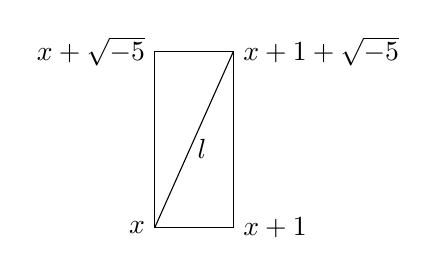
\begin{tikzpicture}
\draw (0,0) -- (1,2.24)  node at (.6,1) {$l$};
\draw (0,0) node[left]{$x$}--(1,0)node[right]{$x+1$}--(1,2.24)node[right]{$x+1+\sqrt{-5}$}-- (0,2.24)node[left]{$x+\sqrt{-5}$}--cycle; 
\end{tikzpicture}
\end{center}

Dann ist $\frac{1}{2}l=\frac{1}{2}\sqrt{6}>1$. Daher funktioniert unser Argument für den EUKLIDischen Algorithmus nicht, wie bei es bei $\IZ[i]$ der Fall war. Tatsächlich ist $\IZ[\sqrt{-5}]$ nicht faktoriell, denn in $A$ gilt $21=3\cdot 7=(4+\sqrt{-5})(4-\sqrt{-5})$. Dabei sind alle Faktoren prim.

\begin{Beweis}
 Ist $3=xy$, so ist $9=\N(x)\N(y)$. Ist $\N(x)=1$, dann ist $x$ Einheit. Also o.B.d.A. $\N(x)=\N(y)=3$. Aber $\N(x)=a^2+5b^2=3$ hat keine Lösung in $\IZ$ $\lightning$. Also $3$ irreduzibel. Analog ist $7$ irreduzibel, denn $a^2+5b^2=7$ hat keine Lösung in $\IZ$.
 
 Ist $4+\sqrt{-5}=xy$ folgt $\N(4+\sqrt{-5})=21=\N(x)\N(y)$. Auch hier führen $\N(x)=3$ oder $\N(x)=7$ zum Widerspruch. Also $4\pm \sqrt{-5}$ irreduzibel.
 
 Wir zeigen: $3,7$ und $4\pm\sqrt{-5}$ sind alle nicht prim. Es genügt zu zeigen, dass für $x\in\{3,7,4\pm\sqrt{-5}\}$ das Ideal $(x)$ kein Primideal ist, also $A/(x)$ kein Körper ist.
 \begin{align*}
  \IZ[\sqrt{-5}]/3\IZ[\sqrt{-5}] &= \IF_3 \oplus \sqrt{-5}\IF_3\\
  &= \IF_3[T]/(T^2+5)\\
  &= \IF_3[T]/(T^2-1) \,(5=-1 \mbox{ in } \IF_3)\\
  &= \IF_3 \oplus \IF_3
 \end{align*}
Analog für $7$: $T^2+5=T^2-2=(T-3)(T+3)$ in $\IF_7[T]$.

$(4+\sqrt{-5})\IZ[\sqrt{-5}]$ hat folgenden Index in $\IZ[\sqrt{-5}]$:
\[\left| \det \begin{pmatrix}
               4 & -5\\
               1 & 4
              \end{pmatrix}
 \right|, \]
 denn der Index der Untergruppe ist gerade die Anzahl aller Elemente aus $\IZ[\sqrt{-5}]$ (\glqq Volumen\grqq) in einem $(4+\sqrt{-5})\IZ[\sqrt{-5}]$-Kästchen. Dazu berechnen wir also die Determinante der Basistransformationsmatrix von 
 \[B=(1,\sqrt{-5})\hspace{5mm} (\IZ\mbox{-Basis von }\IZ[\sqrt{-5}])\] 
 nach 
 \[C=(4+\sqrt{-5},\sqrt{-5}(4+\sqrt{-5})=-5+4\sqrt{-5})\hspace{5mm} (\IZ\mbox{-Basis von }(4+\sqrt{-5})\IZ[\sqrt{-5}]).\]
 Also erhalten wir Index 21. Folglich hat $A/(4+\sqrt{-5})A$ Ordnung $21$ (analog für $4-\sqrt{-5}$).
 
 Es gibt keinen Körper der Ordnung $21$, denn jeder endliche Körper hat einen Primkörper mit Primzahlcharakteristik $p$ und bildet über diesem einen Vektorraum mit $p^k$ Elementen. Aber $21\neq p^k$. 
\end{Beweis}

\begin{Bemerkung}
In den nächsten Wochen beschäftigen wir uns damit die Eindeutigkeit der Zerlegung in solchen Ringen zu retten. KUMMERs Idee dazu war, ideale Zahlen zum Ring hinzuzufügen, sodass $3,7$ und $4\pm\sqrt{-5}$ weiter zerfallen und man die Eindeutigkeit der Primfaktorisierung zurück gewinnt. 
\end{Bemerkung}